\begin{figure}[t]
    \centering
    \def\svgwidth{\columnwidth}
    \fontsize{10}{10}\selectfont
    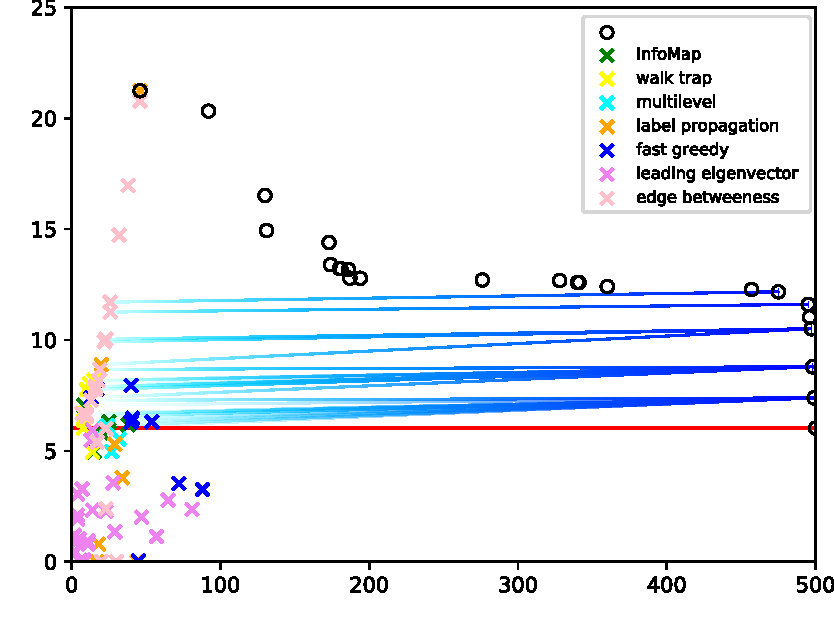
\includegraphics[width=\linewidth]{abcomm}
    \hfill
    \vspace{-.5em}
    \caption{
   		 Strength versus size plots showing existing algorithms fail to give strong communities of
		 large sizes. We use an LFR benchmark network~\cite{lancichinetti2009benchmarks} generated
		 with $\mu=0.1$. Each black circle is a community obtained by our method at $\beta = 0.9$ and
		 each {\sffamily x}-mark is a community obtained by another method.
		 %A blue line connects a community returned by other methods to community returned by our method if the former has weaker strength and is contained in the later.
		 %A blue line connects an {\sffamily x}-mark to a circle if the community of former is contained in the latter and has weaker strength.
		 A blue line connects an {\sffamily x}-mark to a circle if the community of former has weaker strength and is contained in the latter.
		 All points below the red line (shaded in grey) are dominated by the trivial community consisting of all the nodes.
    }

  \label{fig:LFR}
\end{figure}


